\documentclass[12 pt]{article}
\usepackage{amssymb,amsmath,amstext,amsgen,amsbsy,amsopn,amsfonts,graphicx,theorem, anysize,multicol,algorithm, algorithmic, CJKutf8, url,setspace}
%\marginsize{0.5in}{0.5in}{0.5in}{0.5in}
%\marginsize{left}{right}{top}{bottom}
%\usepackage[lmargin=2cm,,rmargin=2cm,tmargin=2cm,bmargin=2cm]{geometry}
\usepackage[margin=1.2in]{geometry}

\begin{document}
\bibliographystyle{acm}
\title{CP4101 HYP Interim Report \\ Citation Provenance\footnote{Project Code: H079820}}
\author{Heng Low Wee \\ U096901R}
\maketitle

\doublespacing
\section{Introduction}
\paragraph{}
Citing previously published scientific papers is a necessary and common practice among researchers. It gives credit and acknowledgement to original ideas, and to researchers who did significant work in a particular field of research, and more importantly, upholds intellectual property. A reader of such research papers often encounters these citations made by the authors in various sentences throughout the paper. Often enough, if a reader wishes to gain a better understanding of the current context, it is necessary to follow through these citations and read up on these cited papers. Readers would also be interested to know where the information is in the cited paper.

\subsection{The Problem}
\paragraph{}
Readers would read up on the cited papers to gain a better insight on the current topic of discussion. However, as frequent readers might find, most citations are only \textit{mentions}. They do not directly refer to some particular section of the cited paper, for example, to make reference to the evaluation results made by the authors of the cited paper. Instead, they are general citations. These citations are important. However since it is not immediately clear where the cited information is from, a reader has to invest additional time to read through the entire cited paper before being able to find out what or where the critical information is. The difficulty is increased when the cited document is a research journal, where the amount of content is comparably huge. The author might specify using the journal's volume number, issue and page number, but the problem remains. This practice makes little contribution to a reader's understanding of the current topic, and it is also time-consuming.

\subsection{Our Goal}
\paragraph{}
In general, we wish to improve the reading experience of scientific \& research documents, from the various fields of research. We want to provide information about the provenance of a citation made in a paper. Readers will be informed of where exactly the cited information is from in the cited paper. We aim to be able to perform this \textit{locating} task accurately. For instance, if a citation is made to refer to the evaluation results computed by the authors of the referenced paper, the reader would be \textit{guided} to the particular section of that paper. By \textit{guiding}, we refer to having the section with the critical information highlighted so the reader can quickly read up on it, before resuming on the current paper. If the citation was a general citation, the reader will be referred to the Abstract section of the paper.

\paragraph{}
We want to develop a reading tool for readers of scientific papers. This reading tool will be able to provide the reader with information about the cited papers, and depending on whether the citations are general or specific, the contents of the cited paper will highlighted accordingly, so that reader may make a quick reference to the cited paper without interrupting the current reading.

\paragraph{}
With the above in mind, we investigate the following related works.

\section{Related Work}
\subsection{Helping Users Make Relevance Judgements About Cited Documents}
\paragraph{}
Practitioners and researchers often have very little time to read lengthy scientific papers, however it is also necessary for them to do so in order to keep themselves updated on the latest developments in their fields of work. Wan et al.\cite{citation-sensitive} investigated the \textit{literature browsing task} by conducting surveys on researchers who read scientific papers frequently to update themselves. In this initial study conducted by Wan et al., several key ideas were revealed. First, when researchers read scientific papers and see citations made by the author, their main concern, as time-constrained professionals, is whether the cited paper would be worth their time and effort, and money, to follow up on and at the same time, whether to believe in the citation. Second, readers faced the difficulty of finding the exact text that justify the citation. Third, the surveys revealed that readers found it useful if a reading tool could identify important sentences and key words in the cited paper.

\paragraph{}
This study conducted by Wan et al. is based on the fundamental idea of improving the reading experience of practitioners and researchers. The goal is to save a reader's time by helping the reader make relevance judgements about the cited documents. As it is often that readers have to read up on the cited documents to gain a better insight on the current context, this task would be of relevance. The authors then developed the CSIBS\cite{csibs} based on their studies. The CSIBS tool helps reader determine whether to read on the cited papers by providing a contextual summary of the cited papers.

\paragraph{}
We are interested in the conclusions drawn from this study conducted by Wan et al. In our project, our goal is also to be able to locate the exact phrases and sentences that would validate a citation made by an author. The CSIBS provides readers contextual previews to help them justify the citation. In our project, we aim to extend this feature, and be able to provide the \textbf{actual} cited information accurately. Another key idea learnt was to be able to identify key words in the cited document. For a reader who has little time to read the entire text, it is useful for the reader to identify first what are the key points in the cited document before investing on reading the entire text.

\subsection{Identifying Keywords In A Document}
\paragraph{}
Much work has been done on automated extraction of keywords from documents. In Hulth\cite{keywordextraction_ml}'s work, instead of the straightforward way of determining keywords by means of term frequency, she showed that by adding linguistic knowledge it could improve the automated process of keyword extraction. In that paper, Hulth adopted a supervised machine learning approach to perform automated keyword extraction. In a later work, Hulth\cite{keywordextraction_mlnlp} combined machine learning techniques and natural language processing to perform automated keywords extraction. On the other hand, Zhang\cite{keywordextraction_crf} introduced an approach to keyword extraction using CRF. In that work, Zhang demonstrated that using the CRF model outperforms other machine learning methods such as SVM. Matsuo \& Ishizuka\cite{keywordextraction_corpusfree} presented a new keyword extraction algorithm that could be applied to a single document without the need of a corpus. In that work, they studied the importance of terms in the document by studying the co-occurrence distribution of terms in a document.

\paragraph{}
We are interested in works related to automatic keywords identification because we want to be able to locate the keywords in a document, particularly the documents cited by a paper. Since keywords in a document are also the most important terms in that document, these keywords would reside within the critical sections of the paper. Intuitively, a scientific paper is cited for its key ideas and findings, it is logical to conclude that these ideas are illustrated with the keywords. Identifying keywords in a document is an important feature that informs the reader what are the key ideas described in the cited paper, and could help the reader identify where the critical information is, and then to justify whether the citation is relevant. Nguyen \& Kan\cite{keyphrase} presented an algorithm for key phrase extraction from scientific publication. A useful feature in their work was capturing the positions of key phrases in documents. We also highlight the work by Matsuo \& Ishizuka, because their algorithm was able to achieve results comparable to a \url{tf-idf}\cite{irtextbook} implementation. This presents a corpus-independent approach, even though the importance of terms is not determined by the field in which the paper belongs to.

\section{Progress So Far}
\subsection{Analysing The Problem}
\subsubsection{Types Of Citation}
\paragraph{}
In the scope of our project, all citations could be classified into 2 types: General, and Specific. We define citations as such to be inline with our goal. That is, to be able to tell, if specified, where the cited information is in the cited document. Otherwise, the citation would be deemed general. A general citation is essentially a \textit{mention}, and the author is making reference to a paper as a whole, usually because the cited paper is of the same field of study. A specific citation is more direct. It refers to a particular section, paragraph, or even line of the cited paper. For example, this often happens in the case where the author wishes to refer to some development by the cited authors, or to make reference to the evaluation results in order to compare performance. In the field of Computer Science, it is often authors make reference to some particular computer system, or some computing algorithms, and to compare performance on speed \& accuracy on solving problems.

\subsubsection{Locating The Cited Information}
\paragraph{}
Our problem can then be reduced to determining whether a citation is General or Specific. If a citation is general, the reader can be directed to the Abstract section of the cited paper. If a citation is specific, the reader can be directed to that specific paragraph or lines respectively. Therefore during computation, the cited document can be broken down into \textit{fragments}. We define a \textit{fragment} as a chunk of $k$ lines of the paper. Hence if given that a citation is specific, then there must exists a fragment that the citation refers to. For this we need to implement some ranking system that determines the location of this fragment. And if the ranking system is unable to determine a \textit{best} fragment, then the citation is probably a general one.

\subsubsection{Scope Of The Problem}
\paragraph{}
In this project, we assume that we are already know of the list of citations made by a paper. Clearly, this coincides with the References/Bibliography section of any paper. We abstract away the problem of locating the in-line citations in a paper, and reduce our problem to only determining the type of citations and its location. To solve the problem of locating the in-line citations, we utilize the open-source ParsCit\cite{parscit} system developed by Councill et al. Conveniently, ParsCit provides the sentence that contains the citation, and these surrounding words would provide us with the context of the cite.

\paragraph{}
We will focus on determining the nature of citations, and its location in the cited document. After computing for the location of the cited information, the output of our application would be a visual display highlighting the cited information.

\subsection{Modeling The Problem As Search}
\paragraph{}
In web search engines, an user enters a search query, and a search engine would use this query to search within its search domain -- millions of web pages -- and then display the best matching web pages as compared to the search query. That would be equivalent to having a search query for an entire corpus of research papers. Our problem can also be modeled as a searching problem, but a reduced version as compared to web search engines.

\paragraph{}
Consider reading a paper, \url{A}. We know the citations made by \url{A}, and these cited papers are listed in the References section of \url{A}. From this our search domain for any query from \url{A} would be the contents of the list of cited papers. We reduce this search domain further when we are investigating a particular citation in \url{A}, say now paper \url{A} cites the paper \url{B}. Now, for this citation, the scope of search would be the sub-domain -- contents of paper \url{B}. So instead of searching for the best matching document in the corpus, we are now searching within \url{B}. Our problem analysis tells that we have to break down \url{B} into fragments, and the search query would be for these fragments (Refer to Figure \ref{fig:model} for a simple illustration). With the help of ParsCit\cite{parscit}, the sentence that contains that cite can be extracted. The search query would then be made up of the surrounding words around the citation.

\begin{figure}[h]
  \centering
  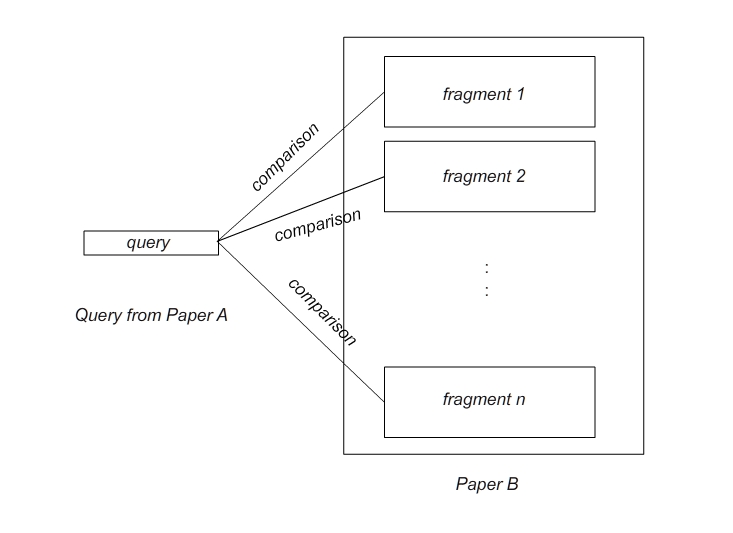
\includegraphics[scale=0.75]{./model}
  \caption{Modeling Our Problem}
  \label{fig:model}
\end{figure}

\subsection{Tackling The Problem}
\subsubsection{Training Corpus}
\paragraph{}
At this initial stage, we picked the ACL Anthology Reference Corpus\footnote{http://acl-arc.comp.nus.edu.sg/} (ACL-ARC). The ACL-ARC consists of publications of the Computational Linguistics field. Note that in general, we wish to perform this citation provenance task on all publications from all fields of research. This corpus is chosen as a start, because it provides the interlink data that conveniently informs us of the citation-links between the papers in the corpus. For instance, in the interlink data, a link like \url{X98-103 ==> X96-1049} says that the paper \url{X98-103} cites \url{X96-1049}.

\subsubsection{Baseline}
\paragraph{}
In the first iteration of the baseline, the idea was to naively compare the search query by term matching frequency. Paper \url{B} will be divided into overlapping fragments of 5 lines, and then each fragment would be compared with the search query. However, common terms like \textit{to}, \textit{the}, \textit{is}, \textit{in} etc. would get high matching frequency, and the results would be definitely skew towards fragments with high number of such terms. These results would not be accurate in general.

\paragraph{}
In the next iteration, we adopted a common mechanism used by search engines, that is to compare the search query and domain for Cosine Similarity\cite{irtextbook}. In our problem, instead of comparing the query with a full document, we are comparing the query with fragments of the target paper. First, we collected the vocabulary set, $V$, using terms from the entire corpus. This is essential because during the comparison for cosine similarity, both vectors must have equal number of dimensions. Each dimension is represented by each unique term in $V$. Both the query and the fragment will be converted into vectors, $v_q$ and $v_f$ respectively.

\paragraph{}
We begin with assigning term frequencies to $v_q$ and $v_f$. Initial tests revealed that common terms affected the comparison results and returned fragments that are not meaningful to be cited.. It becomes necessary we adopt the \url{tf-idf} weighting scheme in order to prevent the commons word affecting the comparison results. \url{tf} simply refers to \textit{term frequency} in a document, while \url{idf} refers to the inverse of the \textit{document frequency} of a term. The \url{df} of a term refers to the number of documents in the corpus that contains that term.
\begin{equation}
\text{\url{tf-idf}}_{t,d} = \text{\url{tf}}_{t,d} \times \log{\frac{N}{\text{\url{df}}_t}}, N=\text{no. of documents in corpus}
\end{equation}
\paragraph{}
By using this weighting scheme, the terms that appear rarely -- with high \url{tf-idf} value -- are \textit{important}, whereas common terms that occur often, like \textit{the} and \textit{to}, are not. This is feasible, since in general, terms that appear often are less important, and we do not want non-important terms to affect our results.

\paragraph{}
We implemented the algorithms for computing \url{tf-idf} and cosine similarity. We pre-prepare information such as $V$, our vocabulary set, \url{tf} for each term with respect to each document, and \url{df} for each term in $V$. In addition, we performed word stemming on the entire corpus. We aimed to speed up computation by pre-preparing these information, since they remain constant for the same corpus.

\section{What's Next}
\label{whatsnext}
\subsection{Gold-Standard Annotations}
\paragraph{}
Using the same corpus, we plan to recruit human participants to gather gold-standard annotations for the research papers. It is essential that we obtain the \textit{correct} locations of cited information, even though it is costly to have humans perform manual annotating on the papers. Only with gold-standard annotations then we can accurately measure the performance of our application. We will annotate for each cite as stated in the interlink data, whether each cite is a general or specific cite. We are particularly interested in specific citations, for that is the goal of our project -- to determine citation provenance and if possible, show exactly where the information is from. Annotations for specific citations should be done down to the level of line numbers of the research paper. For instance, if the cited information appears between line 23 and 28, the annotation should capture it as \url{23-28}.

\paragraph{}
The current state of the corpus do not provide such detailed annotations, and hence it is necessary we conduct such data gathering process. Also, in order to introduce a machine learner component to the application, we would require gold-standard annotations to \textit{train} on.

\paragraph{}
To collect the annotations, we consider two approaches. The first approach is to conduct data gathering sessions in campus and the target participants are students. In each session, each participant would be provided the following:
\begin{enumerate}
\item An annotation file. This file contains the citation-link, and participants will have to annotate whether the citation is General or Specific.
\item The respective research text files. These research text files will be those listed in the annotation file. Participants will have to read through these files to determine the annotation.
\end{enumerate}
To aid the participants on understanding the task, an instructional document, together with some sample annotations and research papers would also be provided to them.

\paragraph{}
The other approach is to use the Amazon Mechanical Turk (MTurk\footnote{https://www.mturk.com/mturk/welcome}). Online participants will also be provided the same set of documents to allow them perform the task. One reason for opting to use MTurk is it provides tools and guidelines that conveniently helps us manage our data collection on this online platform. Another reason is its outreach to large number of participants and would allow us to collect large amount of data. Our principal consideration, however, is we have to filter our target participants as we do require them to be able to understand the contents on the research papers.

\subsection{NLP Component}
\paragraph{}
It is a common practice for authors, when citing another paper, to paraphrase the original sentences, often to achieve greater clarity for the current context. Naturally, the terms in the paraphrase would be different from the original sentence written in the cited paper. The baseline we used is still a frequency-based technique to determine the importance of terms in the document. Queries are not context-sensitive, and so the result might not be able to retain similar context. Furthermore, the baseline would simply treat paraphrased queries as a mis-match. Therefore, we have to explore NLP techniques and mechanisms in order to handle paraphrasing. Shinyama et al.\cite{paraphrase2} described an approach to perform automated paraphrase acquisition from news articles, based on the scenario that these news articles are reporting on the same event. In our context, the citing and the cited papers generally belong to the same topic. We may explore such similar approaches to tackle the paraphrasing problem.

\singlespacing
\bibliography{bibsource}
\end{document}
